\section{Les signaux}

\subsection{Définition}

Commençons par introduire la notion de signal. On appelle \textbf{signal analogique} ou \textbf{continu}, une fonction de $\mathbb{R}$, représentant le temps, vers $\mathbb{C}$ \cite{wiki-signal} . Bien que les mesures physiques soient réelles, un signal complexe permet de conserver la \textbf{phase} au travers de son argument et son \textbf{amplitude} au travers de son module.

    \begin{figure}[H]
        \caption{Parties réelle et imaginaire d'un signal complexe\cite{sinusoidal}}
        \begin{center}
        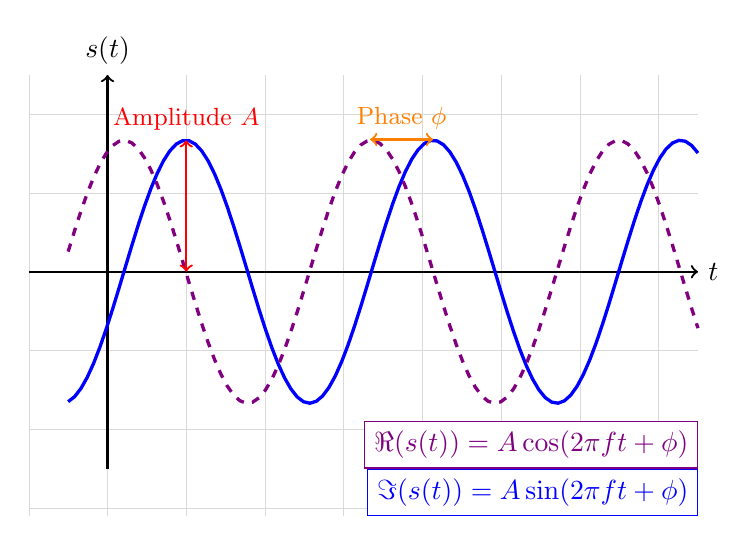
\begin{tikzpicture}
            \draw[very thin, gray!30] (-1,-3.1) grid (7.5,2.5);
            \draw[->, thick] (-1,0) -- (7.5,0) node[right] {$t$};
            \draw[->, thick] (0,-2.5) -- (0,2.5) node[above] {$s(t)$};
            
            \draw[blue, very thick, samples=100, domain=-0.5:7.5] 
                plot (\x, {1.67*sin(deg(2*\x - 6.7))});
            
            \draw[violet, very thick, dashed, samples=100, domain=-0.5:7.5] 
                plot (\x, {1.67*cos(deg(2*\x - 6.7))});
            
            \draw[red, <->, thick] (1, 0) -- (1, 1.67) 
                node[above, above, font=\small] {Amplitude $A$};
            
            \coordinate (Origin) at (0, 0.5);
            \coordinate (Peak) at (0.4, 0.5);
            
            \draw[orange, <->, thick] (3.335, 1.68) -- (4.135, 1.68) 
                node[midway, above, font=\small] {Phase $\phi$};
            
            \node[violet,draw, fill=white, anchor=south east] at (7.5, -2.5) 
                {$\Re (s(t)) = A\cos(2 \pi f t + \phi)$};
                
            \node[blue,draw, fill=white, anchor=south east] at (7.5, -3.1) 
                {$\Im (s(t)) = A\sin(2 \pi f t + \phi)$};
        \end{tikzpicture}
        \end{center}
    \end{figure}

    \vspace{0.5cm}

Le signal $s(t) = A e^{i(2\pi ft + \phi)}$ représenté ici est un signal dit "pur". En réalité, la plupart des signaux ont des formes beaucoup plus complexes et ne ressemblent pas à une simple sinusoïde. 

Le traitement numérique du signal nécessite une discrétisation pour y appliquer des algorithmes informatiques.

\subsection{Échantillonnage}
\label{section-echantillonnage}

Les signaux analogiques décrits précédemment ne peuvent pas être traités numériquement tels quels. L'échantillonnage est le processus permettant de passer d'un signal analogique à un signal numérique. Il consiste en la sélection d'un nombre fini de valeurs du signal analogique pour constituer un vecteur de coefficients représentatif du signal.

Pour ce faire, on choisit un intervalle de temps, que l'on découpe en $N$ sous-intervalles de longueur $T$. L'échantillonnage correspond alors à conserver uniquement les valeurs du signal aux temps $nT$ pour $T \in \{0, \dots, N - 1\}$ (\hyperref[preuve-echantillonnage]{Voir le procédé détaillé en annexe}). On peut alors considérer ce signal échantillonné fini comme un vecteur :
\begin{align*}
    x = (s(0),s(T),s(2T),...,s((N-1)T)) =  (x_0,x_1,...,x_{N-1}) \in \mathbb{C}^N
\end{align*}

On peut alors appliquer des traitements numériques à $x$, le signal échantillonné de $s$.

\begin{figure}[H]
    \caption{Échantillonnage d'une fonction continue}
    \begin{center}
        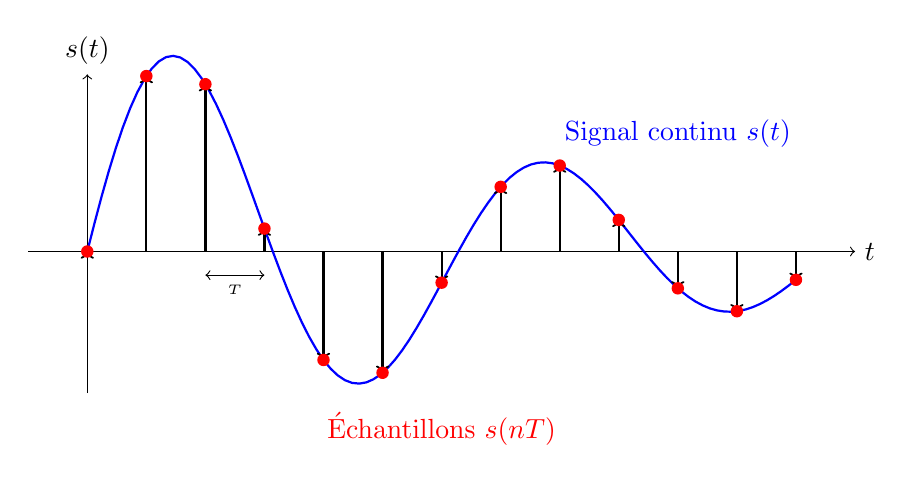
\begin{tikzpicture}[scale=1.5]

        \draw[->] (-0.5,0) -- (6.5,0) node[right] {$t$};
        \draw[->] (0,-1.2) -- (0,1.5) node[above] {$s(t)$};

        \draw[thick, blue, domain=0:6, samples=100] 
            plot (\x, {2*exp(-\x/4)*sin(2*\x r)});
        \node[blue] at (5,1) {Signal continu $s(t)$};

        \foreach \x in {0, 0.5, ..., 6} {
            \pgfmathsetmacro{\y}{2*exp(-\x/4)*sin(2*\x r)}
            \draw[->, black, thick] (\x, 0) -- (\x, \y);
            \fill[red] (\x, \y) circle (1.5pt);
        }
        \node[red] at (3,-1.5) {Échantillons $s(n T)$};
        \draw[<->] (1, -0.2) -- (1.5, -0.2) node[midway, below, font=\tiny] {$T$};
    \end{tikzpicture}
    \end{center}
\end{figure}
